\newpage
\begin{center}
  \textbf{\large 1. Аналитический обзор }
\end{center}
\refstepcounter{chapter}
\addcontentsline{toc}{chapter}{1. Аналитический обзор }

\section{Использование подходов ИИ в робототехнике}

    В последнее время, методы искусственного интеллекта показывают выдающиеся результаты в решении различных робототехнических задач, таких как: манипуляция \cite{related-manipulation-1, related-manipulation-2}, передвижение квадропедов \cite{related-locomotion-1, related-locomotion-2}, управление дронами \cite{related-drone-1, related-drone-2}, многоагентное планирование \cite{related-multi-agent-1, related-multi-agent-2} и многих других. Выделяют два основных подхода обучения моделей искусственного интеллекта в робототехнике: обучение с подкреплением (англ. Reinforcment Learning) и имитационное обучение (англ. Imitation Learning). 

    \subsection{Обучение с подкреплением}

        Обучение с подкреплением (Reinforcement Learning, RL) — это обширная область исследований, изучающая автономное принятие последовательных решений.

        В формальной постановке задачи обучения с подкреплением существует агент (англ. agent), который взаимодействует с окружающей средой (англ. environment), принимает действия (англ. actions). За каждое действие агент получает награду (англ. reward) от среды. Агент задаёт процедуру выбора действия на основе текущего состояния среды, эта процедура называется стратегией (англ. policy). Целью агента является максимизация кумулятивной награды.  
        
        Постановка задачи обучения с подкреплением опирается на определение марковского процесса принятия решений (МППР) \cite{puterman2014markov}:

        \begin{itemize}
            \item пространство состояний $S$ 
            \item множество действий $A$
            \item $T: S \times A \to S$ -- функция переходов
            \item $R: S \times A \to \mathbb{R}$  -- функция вознаграждений
            \item $\gamma$ -- дисконтирующий множитель
        \end{itemize}

        Агент выполняет действие в среде, используя функцию стратегии (\ref{eq:policy}): 

        \begin{equation}
            \pi: S \to A.
            \label{eq:policy}
        \end{equation}

        В момент времени $t$ агент находится в состоянии $s_t \in S$, выбирая действие $a_t = \pi(s_t), a_t \in A$, агент переходит в состояние $s_{t + 1}$ исходя из распределения $p(s_{t + 1} | s_t, a_t)$, задающимся функцией перехода $T$, и получает награду $r_t = R(s_t, a_t)$. Суммарное дисконтированное вознаграждение имеет вид (\ref{eq:cum_reward}): 

        \begin{equation}
            R = \sum_{t = 0}^\infty  \gamma^t r_t = r(s_0, a_0) + \gamma r(s_1, a_1) + \gamma^2 r(s_2, a_2) \dots
            \label{eq:cum_reward}
        \end{equation}

        Тогда, формальная цель агента -- максимизировать ожидаемую отдачу по стратегии $\pi$ (\ref{eq:agent_goal}):

        \begin{equation}
            \mathbb{E}_{\pi} \sum_{t = 0}^\infty \gamma^t r_t.
            \label{eq:agent_goal}
        \end{equation}

        В большинстве реальных систем, агент не имеет полного доступа к информации о состоянии среды $s_t$ в каждый момент времени, вместо этого он получает от среды наблюдение (англ. observation) $o_t \in O$. Такой процесс называется частично наблюдаемым марковским процессом \cite{kaelbling1998planning}.

        Функция полезности состояния -- это ожидаемое дисконтированное кумулятивное вознаграждение, которое получит агент следуя стратегии $\pi$ из состояния $s$ (\ref{eq:V}):

        \begin{equation}
            V^{\pi} (s) = \mathbb{E}_{\pi} \left[ \sum_{i = 1}^{\infty} \gamma^i r(s_{t + i}, a_{t + i} | s_t = s) \right].
            \label{eq:V}
        \end{equation}

        Функция полезности действия -- это ожидаемое дисконтированное кумулятивное вознаграждение получаемое агентом при использовании действия $a$ в данном состоянии $s$ и стратегии $\pi$ для будущих состояний в эпизоде (\ref{eq:Q}):

        \begin{equation}
            Q^{\pi} (s, a) = \mathbb{E}_{\pi} \left[ \sum_{i = 1}^{\infty} \gamma^i r(s_{t + i}, a_{t + i} | s_t = s, a_t = a) \right].
            \label{eq:Q}
        \end{equation}

        
    \subsection{Имитационное обучение}

        Постановка задачи имитационного обучения схожа с постановкой задачи обучения с подкреплением, основное отличие заключается в том, что вместо использования явной функции вознаграждения $r_t = R(s_t, a_t)$ предполагается наличие набора демонстраций, предоставленных экспертом.

        Если, в рамках парадигмы МППР, есть среда с функцией переходов $T: S \times A \to S$, с состоянием $s \in S$ и действием $a \in A$, то задача имитационного обучения заключается в использовании набора демонстраций $\Xi = \{ \xi_1, \dots, \xi_D\}$ экспертной стратегии $\pi^*$, для нахождения стратегии $\hat{\pi}^*$, которая имитирует экспертную стратегию.

        Одним из наиболее популярных методов имитационного обучения является подход клонирования поведения (англ. Behavior Cloning). Данный метод использует набор экспертных демонстраций $\xi \in \Xi$, чтобы определить стратегию $\pi$, которая бы имитировала эксперта. Это задача может быть решена в рамках задачи обучения с учителем, где разница между выходом стратегии и экспертными демонстрациями минимизируется относительно некоторой метрики. Формально, цель -- решить оптимизационную задачу (\ref{eq:bc}):

        \begin{equation}
            \hat{\pi}^* = argmin_{\pi} \sum_{\xi \in \Xi} \sum_{s \in \xi} L (\pi(s), \pi^*(s)),
            \label{eq:bc}
        \end{equation}

        где $L$ - функция потерь, $\pi^*(s)$ -- действие экспертной стратегии в состоянии $s$, $\pi^*$ -- аппроксимированная стратегия. 

        Ограничение применения подхода клонирования поведения заключается в том, что обучение происходит исключительно за счет экспертных демонстраций, которые могут неравномерно покрывать всё пространство состояний, а так же они могут быть не оптимальными с точки зрения некоторого функционала качества
        

\subsection{Обучение на синтетических данных}

    В рассмотренных выше подходах машинного обучения, среда может быть реальной или симуляционной. Симуляционная среда, симулятор -- это программно-моделируемое виртуальное пространство, которое с заданной точностью воспроизводит физические законы, динамику объектов и сенсорные данные реального мира.

    Использование симуляторов в контексте применения методов машинного
    обучения в робототехнике обусловлено ресурсоёмким и небезопасным
    процессом сбора данных или взаимодействием со средой в реальных условиях. Альтернативой такому подходу выступает генерация данных в симуляторе, где данные дешевые, а взаимодействие агента со средой и сбор данных не угрожает реальному оборудованию и персоналу. Несмотря на преимущества, основной проблемой данного подхода является так называемая проблема sim-to-real gap \cite{he2023bridging}. Данная проблема обусловлена тем, что симулятор представляет собой модель реального мира, и его воспроизведение процессов отличается от того, как аналогичные процессы происходят в реальности. Вследствие модель во время обучения на данных из симулятора, учится оперировать в мире с одними характеристикам (динамикой, визуальными представлениями и т.д.), а затем запускается в условиях других. Обычно, среда, в которой предполагается функционирование агента, называется целевым доменом, а среда, в которой проходил процесс обучения -- исходным. В рамках проблемы sim-to-real gap: реальный мир -- это целевой домен, симулятор -- исходный домен.  

    Существует множество решений описанной проблемы такие как: идентификация системы \cite{sontakke2023residual}, доменная рандомизация \cite{dai2022analysing, shakerimov2023efficient}, доменная адаптация \cite{shakerimov2023efficient} и другие. Концептуальные иллюстрации основных подходов изображены на рисунке \ref{fig:sim2real}. 
    
    Идентификация системы заключается в построении точной математической модели реального объекта, данный подход обладает высокой точностью, однако требует значительных ресурсов для реализации. Доменная адаптация предполагает обучение модели на данных из исходного домена для применения в целевом домене. Подразумевается, что полученный моделью опыт на исходном домене должен позволить ей успешно справиться с данными из целевого домена. Подход доменной рандомизации обладает большей популярностью ввиду его простоты. Суть подхода подразумевает создание разнообразных сценариев обучения, путём варьирования параметров симуляции, таких как: физические и визуальные характеристики объектов и окружающей среды, освещение, кинематические и динамические параметры робота и другие. В таком случае, предполагается, что среда реального мира -- это одна из вариаций исходной среды симулятора. Формально, есть заданный набор из $N_{rand}$ параметров симуляции, которые будут рандомизированы. Набор параметров $\xi$ выбирается из пространства рандомизаций $\Xi \subset \mathbb{R}^{N_{rand}}$, где каждый параметр $\xi^{(i)}$ ограничен отрезком $\left[ \xi^{(i)}_{low}, \xi^{(i)}_{high} \right]^{N_{rand}}_{i=1}$. В начале каждого эпизода генерируются параметры $\xi \in \Xi$ и передаются симулятору $S$, по которым генерируется среда $E$. Полученная среда используется для обучения стратегии агента $\pi$. В контексте МППР, под воздействием доменной рандомизации могут быть изменены составляющие пространство состояний $S$, множество действий $A$ и функция переходов $T$, однако награда $R$ и дисконтирующий множитель $\gamma$ остаются неизменными \cite{mehta2020active}. Предполагается, что если модель будет эффективной на распределении вариаций сцен, генерируемой доменной рандомизацией, то она будет эффективна и в реальных условиях. Таким образом доменная рандомизация решает проблему sim-to-real, делая модель более робастной по отношению к различным сценариям.  

    \begin{figure}
        \begin{center}
            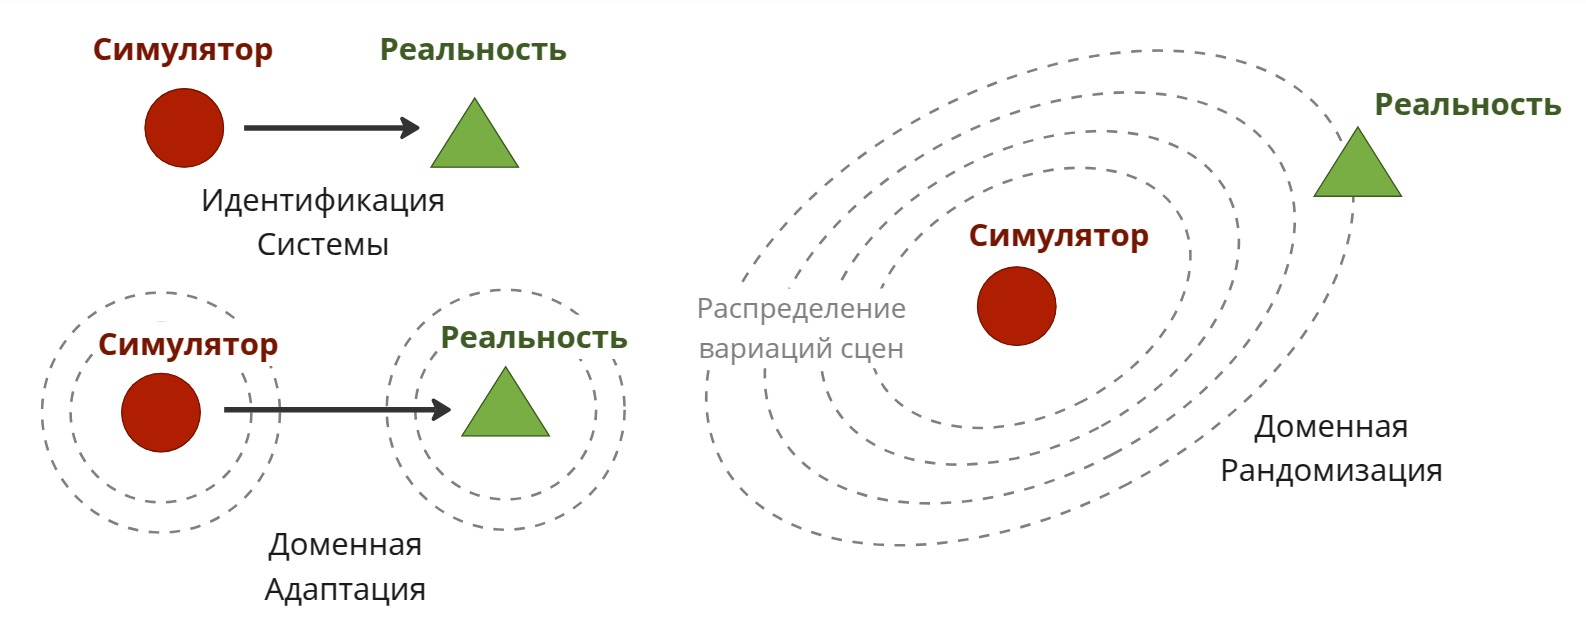
\includegraphics[width=0.8\textwidth]{images/sim2real.jpg}
        \caption{Концептуальные иллюстрации основных подходов решения проблемы sim-to-real \cite{weng2019DR}}
        \label{fig:sim2real}
        \end{center}
    \end{figure}

    \section{Валидация моделей}
    
    Аналогично проблеме обучения на синтетических данных актуальным является вопрос о тестировании моделей в симуляторе. Перед развертыванием любой обученной модели в реальном мире необходимо удостовериться в её способности решать поставленную задачу эффективно и безопасно. Экспериментальные запуски в реальном мире требуют дополнительных ресурсов и не могут в полной мере предотвратить потенциальные угрозы. По этой причине процедура валидации или тестирования моделей в симуляторе является перспективным направлением развития на пути повсеместного использования искусственного интеллекта на реальных робототехнических системах. 

    Естественным подходом в данной области является уменьшение разрыва между симулятором и реальностью, что может быть реализовано, например, посредством синтеза фотореалистичных визуальных данных и применения методов идентификации систем для определения точных параметров модели робота \cite{li24simpler}. Для количественной оценки соответствия эффективности модели в симуляции и в реальных условиях используют метрику Sim-to-Real Correlation Coefficient (SRCC) \cite{kadian2020sim2real}. Однако, данный подход может оказаться дорогостоящим и не масштабируемым, так как требует значительных человеческих ресурсов для построения высокоточной модели реальности в симуляторе. Более того, данный подход не прогнозирует изменение эффективности модели под воздействием возмущающих факторов, присущих среде реального мира.

    Альтернативой или дополнением к описанному подходу выступает метод оценивания робастности моделей. Основная идея заключается в вычислении изменений показателей эффективности модели при различных рандомизациях симуляционной среды, где рандомизации описываются и применяются аналогично методу доменной рандомизации \cite{pumacay2024colosseum, li24simpler}. Таким образом, данный метод оценивает робастность модели относительно возможных внешних возмущений. Далее рассмотрены различные реализации метода.

        \subsection{The Colosseum}
    
        Одним ярким примером такого метода для оценки робастности моделей является работа The Colosseum \cite{pumacay2024colosseum}, целью которого является определение падения эффективности моделей при изменении параметров среды. Метод предоставляет собой программный модуль на базе платформы RLBench \cite{james2020rlbench} позволяющий варьировать 14 параметров среды, среди которых цвета, текстуры объектов, параметры освещения и другие. Эффективность моделей оценивается долей успешных эпизодов, где успешность эпизода определяется задачей. Алгоритм работы метода можно описать следующим образом:
    
        \begin{enumerate}
            \item Генерация обучающего набора данных на исходной, не рандомизированной среде;
            \item Обучение модели на сгенерированных данных, робастность которой будет оцениваться;
            \item Тестирование обученной модели в среде, с последовательным варьированием каждого из 14 параметров;
            \item Для каждого параметра производится расчет падения доли успешных эпизодов относительно доли успешных эпизодов на исходной, не рандомизированной среде;
            \item Определение ключевых для работы модели параметров, варьирование которых сильнее других влияет на эффективность модели.
        \end{enumerate}
    
        По данному алгоритму авторы работы оценили робастность 5 передовых моделей имитационного обучения для манипуляции: R3M \cite{nair2022r3m}, MVP \cite{Radosavovic2022}, PerAct \cite{shridhar2022peract}, RVT \cite{goyal2023rvt}, VoxPoser \cite{huang2023voxposer}. По результатам, доля успешных эпизодов падает на $30-50\%$ при варьировании некоторых параметров среды, и на более $75\%$ при применении всех вариаций. Оказалось, что рассматриваемые модели наиболее уязвимы по отношению к параметрам освещенности, цвету объекта манипулирования и количеству отвлекающих объектов. 

        Также, была установлена корреляция между полученными метриками на реальных и синтетических данных. Таким образом, The Colosseum может быть использован для оценки эффективности модели в реальных условиях под воздействием различных возмущений, однако метод не прогнозирует абсолютное значение эффективности в исходной среде, без возмущений. Также, ограничением данного метода является обучение модели на синтетическом наборе данных, полученных в исходной среде. Такой подход не позволяет оценивать модели, уже обученные на реальных или синтетических данных. 
    
        \subsection{KitchenShift}
            Аналогичный метод предоставляют авторы работы KitchenShift \cite{xing2021kitchenshift}. Отличие от работы The Colosseum заключается в количестве параметров доступных для вариации, в данной работе их 7, среди которых: 3D модели и текстуры объектов, положение камеры, освещение, начальное состояние объектов и робота. Алгоритм выглядит следующим образом:
    
            \begin{enumerate}
                \item Модель обучается задаче $\mathcal{T}_{train}$ в домене $\mathcal{D}_{train}$ с доступом к ограниченному набору демонстраций;
                \item Производится тестирование модели на задаче $\mathcal{T}_{train}$ на множестве доменов $\{\mathcal{D}_{shifted}\}$, которые были получены варьированием параметров среды.
            \end{enumerate}
    
        Согласно этому алгоритму, были оценены методы на основе имитационного обучения, по результатам метрики эффективности моделей значительно снизились под воздействием новых, смещенных параметров среды. Однако, в рамках данной работы не было проведено исследование о корреляции с экспериментами в реальных условиях. Аналогично работе The Colosseum ограничением рассматриваемого метода является обучение модели на синтетическом наборе данных, полученных в исходной среде. 
    
        \subsection{Simpler}
    
            Данная работа \cite{li24simpler} специализируется на оценке робастности уже обученных моделей, она объединяет два описанных подхода, а именно уменьшение разрыва между симулятором и реальностью и применение рандомизаций. Основная идея работы носит имя Visual-Matching и подразумевает увеличение метрики SRCC, посредством создания реалистичной среды с точки зрения визуальных и физических составляющих. Так, были идентифицированы коэффициенты жёсткости и демпфирования сочленений робота на основе реальных траекторий. Для повышенной фотореалистичности текстуры объектов были воссозданы из реальных изображений, как и внешний вид заднего плана. Эмпирическим путем было установлено, что эффективность модели в построенной сцене коррелирует с эффективностью модели в реальном мире. Более того, коррелируют значения падения эффективности при различных рандомизациях, среди которых:~\begin{itemize}
                \item Положение камеры;
                \item Текстура стола;
                \item Отвлекающие объекты;
                \item Освещение;
                \item Задний фон.
            \end{itemize}
            
            Альтернативой вышеописанному методу Visual-Matching в работе был предложен метод Visual-Aggregation, который позволяет предсказывать эффективность модели в реальных условиях, используя тестирование на рандомизациях. Было установлено, что усредненная эффективность модели по рандомизированным средам коррелирует с итоговой эффективностью модели в реальности. Для рандомизации были выбраны следующие параметры:~\begin{itemize}
                \item Освещение;
                \item Задний фон;
                \item Текстура стола.
            \end{itemize}
            
            Каждая рандомизация была ограничена набором из трех заранее определенных вариаций, что не позволяет масштабировать распределение рандомизаций. По этой причине, итоговое распределение сцен в результате рандомизаций не обладает достаточной дисперсией для релевантной оценки эффективности модели. 

            Отмечено, что результаты работы метода Visual-Aggregation имеют меньший коэффициент корреляции, чем результаты работы метода Visual-Matching. Несмотря на это, предложенный метод имеет высокий потенциал, так как имеет более простую реализацию и не требует большого количества данных о реальной среде. 
            
            Таким образом, метод предлагаемый в Simpler, благодаря высокой степени корреляции, позволяет предсказывать эффективность исследуемой модели в реальных условиях, с помощью процесса валидации на рандомизированных средах. 
    
        \subsection{Выводы}

        На примере рассмотренных работ, можно сделать вывод, что метода оценивания робастности на основе рандомизаций достаточно, как для прогнозирования изменения эффективности модели под воздействием внешних возмущений, так и для прогнозирования абсолютной эффективности модели в реальных условиях. Наиболее перспективной является работа The Colosseum, так как она обладает большой масштабируемостью, а также включает в себя большее количество возможных рандомизаций, однако данная работа может быть усилена результатами полученными методом Visual-Aggregation в работе Simpler. 

    \section{Обзор симуляционных платформ для валидации моделей}

    В данном разделе будут рассмотрены перспективные симуляторы для построения метода оценки робастности.

    \subsection{IsaacSim}
    IsaacSim \cite{nvidia_isaac_sim} -- это высокопроизводительная платформа для симуляции и обучения роботов, разработанная NVIDIA. Она позволяет проводить параллельное обучение агентов в виртуальных средах с использованием графических процессоров (GPU). Основные особенности IsaacSim включают:
    \begin{itemize}
        \item Поддержка физически точных симуляций с использованием движка PhysX;
        \item Возможность одновременного обучения тысяч агентов в одной среде;
        \item Высокая реалистичность сцен.
    \end{itemize}
    
    Инструменты предоставляемые IsaacSim позволяют создавать реалистичные сцены, которые упрощают решение проблемы sim-to-real и позволяют проводить оценку моделей, обученных на реальных данных, по примеру работы Simpler.
    
    \subsection{RLBench}
    RLBench \cite{james2020rlbench} -- это платформа для обучения с подкреплением, ориентированная на задачи манипуляции роботами. Она предоставляет набор из более чем 100 задач, таких как открывание дверей, перемещение объектов и сборка конструкций. Особенности RLBench включают:
    \begin{itemize}
        \item Большой набор предопределенных задач, которые можно использовать для тестирования и обучения моделей;
        \item Возможность генерации данных для обучения и тестирования моделей.
    \end{itemize}
    RLBench позволяет оценивать робастность моделей в условиях, близких к реальным, благодаря разнообразию задач и сценариев.
    
    \subsection{MuJoCo}
    MuJoCo \cite{todorov2012mujoco} -- это физический движок, широко используемый для моделирования сложных динамических систем. Основные преимущества MuJoCo:
    \begin{itemize}
        \item Высокая точность моделирования физических взаимодействий, включая контакты, трение и деформации;
        \item Возможность гибкой настройки параметров среды.
    \end{itemize}
    MuJoCo является одной из наиболее популярных платформ благодаря своей гибкости и точности.

    Каждая из рассмотренных платформ имеет свои уникальные особенности, однако, для задачи оценивания робастности наиболее уместным является симулятор IsaacSim, ввиду его повышенной точности и фотореалистичности. 
      